\documentclass{exam}
\usepackage{../../commonheader}
\usepackage{graphicx}
\usepackage{color}

%%% CHANGE THESE %%%%%%%%%%%%%%%%%%%%%%%%%%%%%%%%%%%%%%%%%%%%%%%%%%%%%%%%%%%%%%
\discnumber{}
\title{\textsc{Midterm 2 Review}}
\date{October 12, 2017}
%%%%%%%%%%%%%%%%%%%%%%%%%%%%%%%%%%%%%%%%%%%%%%%%%%%%%%%%%%%%%%%%%%%%%%%%%%%%%%%

\begin{document}
\maketitle
\rule{\textwidth}{0.15em}
\fontsize{12}{15}\selectfont

%%% INCLUDE TOPICS HERE %%%%%%%%%%%%%%%%%%%%%%%%%%%%%%%%%%%%%%%%%%%%%%%%%%%%%%%


%%% Question %%%

\section{List Mutation and Nonlocal}
\begin{questions}

\item Draw the Box and Pointer!
\newline
\begin{lstlisting}
>>> corgi = [3, 15, 18, 7, 9]
>>> husky = [8, 21, 19, 11, 25]
>>> poodle = corgi.pop()
>>> corgi += husky[-3:]
\end{lstlisting}
\begin{solution}
\begin{lstlisting}

\end{lstlisting}
\end{solution}
\vspace{4cm}

\item Draw the Box and Pointer!

\begin{lstlisting}
>>> pom = [16, 15, 13]
>>> pompom = pom * 2
>>> pompom.append(pom[:])
>>> pom.extend(pompom)
\end{lstlisting}

\clearpage
\vspace{4cm}
\item What is the result of calling pop(pip)?

\begin{lstlisting}

pip = [8, 2]
def pop(tart):
    pop = tart[pip[1]:]
    def pup(p):
        nonlocal pop
        pop = [pop.pop()] + [pop] + pop[:] 
        return pop.append(9)
    if pup(3):
        return pop[2]
    return pop[3]
pip.extend([8, 3])
pop(pip)
\end{lstlisting}

\end{questions}
\clearpage

\section{OOP}
\begin{questions}
\item An Energizing Example!
\begin{lstlisting}
class Pokemon:
    hp = 100
    damage = 25
    def __init__(self, name):
        self.name = name
    def attack(self, other):
        other.hp -= self.damage
    def __repr__(self):
        return self.name
 
\end{lstlisting}
For each of the expressions in the table below, write the output displayed by the interactive Python interpreter when the expression is evaluated. The output may have multiple lines. If more than 3 lines are displayed, just write the first 3. If an error occurs, write “Error”. If evaulation would run forever, write “Forever”.\\
Assume that you have started \texttt{python3} and executed the following statements:

\begin{center}
\begin{tabular}{ |p{8cm}|p{6cm}| } 
 \hline
 \begin{lstlisting}
>>> pika = Pokemon('Pikachu') 
>>> pika.hp
\end{lstlisting} &  \\  \hline
 \begin{lstlisting}
>>>pika.damage
\end{lstlisting} &  \\  \hline
 \begin{lstlisting}
>>>pika.trainer = 'Kevin'
>>>pika.trainer
\end{lstlisting} &  \\  \hline
 \begin{lstlisting}
>>>Pokemon.trainer
\end{lstlisting} &  \\  \hline
 \begin{lstlisting}
>>>bulba = Pokemon('Bulbasaur')
>>>bulba.hp -= pika.damage
>>>Pokemon.hp
\end{lstlisting} &  \\  \hline
 \begin{lstlisting}
>>>pika.hp, bulba.hp
\end{lstlisting} &  \\  \hline
\end{tabular}
\end{center}
\clearpage
\begin{center}
\begin{tabular}{ |p{8cm}|p{6cm}| } 
 \hline
 \begin{lstlisting}
>>>pika.attack(bulba)
>>>pika.hp, bulba.hp
\end{lstlisting} &  \\  \hline
 \begin{lstlisting}
>>>Pokemon.attack(pika, bulba)
\end{lstlisting} &  \\  \hline
 \begin{lstlisting}
>>>pika.hp, bulba.hp
\end{lstlisting} &  \\  \hline
 \begin{lstlisting}
>>>pika.attack = lambda self, other: print("It doesn't affect " + other.name)
>>>pika.attack(bulba)
\end{lstlisting} &  \\  \hline
 \begin{lstlisting}
>>>pika.attack
>>>pika.attack = bulba.attack
>>>pika.attack(bulb)
>>>pika.hip, bulba.hp
\end{lstlisting} &  \\  \hline
 \begin{lstlisting}
>>>pika.attack
\end{lstlisting} &  \\  \hline
\end{tabular}
\end{center}


\clearpage
\item ElementPointer
 
 \begin{lstlisting}
 
"""Let's build a class ElementPointer* to keep track of the next element in a list: [1, 2, 3].
Our class will yield the next element upon command.
Our class also allows us to mark a point in our list so that ElementPointer yields the element at that point when we ask for the next element in our list.

*This question is adapted from CS186. '"""

class ElementPointer:

	lst = [1, 2, 3]
	
	def __init__(self):
	
		self.curr_index = 0
				
		self.marked_index = -1

def has_next(self):
		
		"""has_next returns True when there is another element in our list that has yet to be yielded.
		
		>>> a = ElementPointer()
		
		>>> a.next_elem()
		
			1
		
		>>> a.has_next()
		
			True		                           """
		
		____________________________________
		
 def next_elem(self):
		
		"""next_elem returns the next element of the list.
		
		>>> a = ElementPointer()
		
		>>> a.next_elem()
		
			1
		
		>>> a.next_elem()
		
			2                                      """
		
		____________________________________
		
		____________________________________
		
		____________________________________
        
def mark(self):
		
		"""mark remembers the current index of our iterator so that we can reset
		
		back to that mark. mark does nothing if the iterator has not yet yielded an
		
		element or has not yielded an element since the last reset.
		
		>>> a = ElementPointer()
		
		>>> a.next_elem()
		
			1	
		
		>>> a.mark()
		
		>>> a.reset()
		
		>>> a.next_elem()
		
			1      """
		
		____________________________________
		
		____________________________________
		
		____________________________________
		
def reset(self):
		
		"""reset resets the iterator such that the next element it yields is at the marked point.
		
		>>> a.next_elem()
		
			1	
		
		>>> a.mark()
		
		>>> a.reset()
		
		>>> a.next_elem()
		
			1 """
		
		____________________________________
		
		____________________________________
		
		____________________________________
		
		____________________________________
\end{lstlisting}

\end{questions}



\section{Linked Lists and Trees}
\begin{questions}
\item For each of the following code fragments, add arrows and values to the object skeletons to the right to show the final state of the program. Single boxes are variables that contain pointers. Double boxes are Links. Not all boxes need be used.\\
\begin{center}
\vspace{1cm}
% 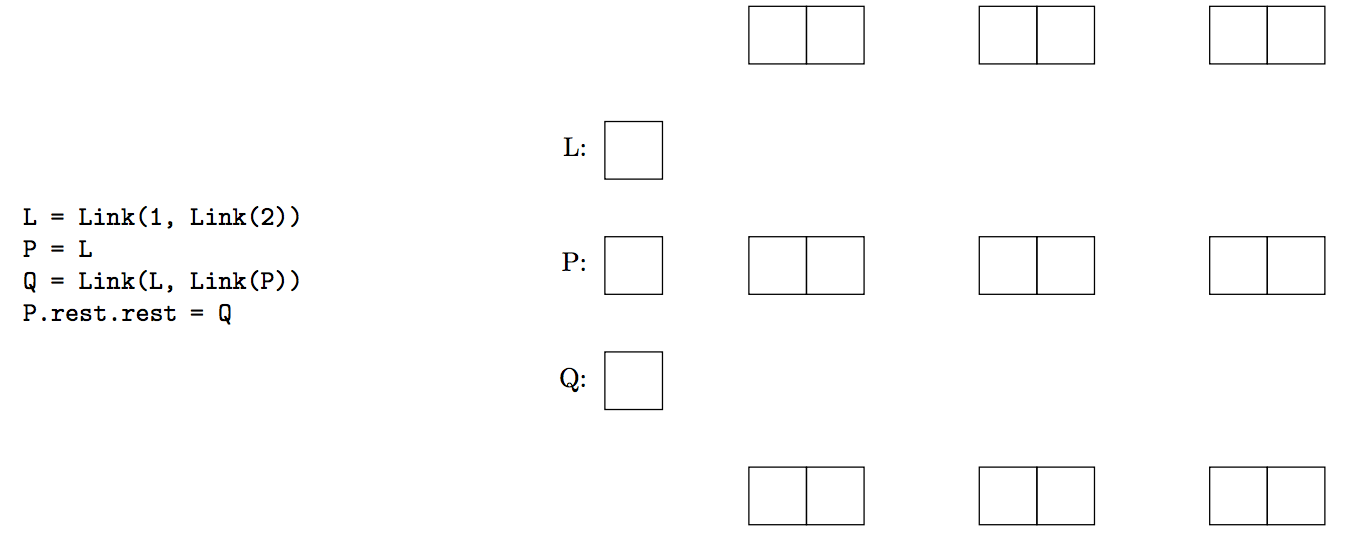
\includegraphics[width=15cm]{a}\\
\vspace{5cm}
 % 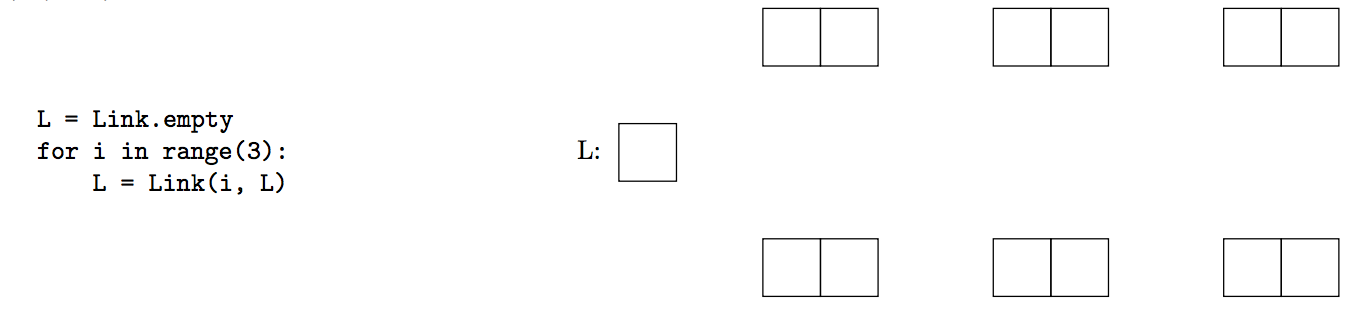
\includegraphics[width=15cm]{b}
\end{center}

\clearpage

\item WWPD? Try drawing a box-and-pointer diagram!
\begin{lstlisting}
def wild(lnk):
    if lnk is Link.empty or lnk.rest is Link.empty:
        return lnk
    breath = wild(lnk.rest)
    lnk.rest.rest = lnk
    lnk.rest = NULL
    return breath
\end{lstlisting}

\begin{center}
\begin{tabular}{ |p{8cm}|p{6cm}| } 
 \hline
 \begin{lstlisting}
>>> triforce = Link(3, Link(1, Link(4)))
>>> wild(triforce)
\end{lstlisting} &  \\  \hline
 \begin{lstlisting}
>>> triforce
\end{lstlisting} &  \\  \hline
\end{tabular}
\end{center}

\item The depth of a node from the root of a tree is measured by its distance from the root. Nodes that have the same depth are said to be on the same 'level'. 
Write a function that returns a dictionary, where each key is a level and each value is a list of all labels on that level. 
 \begin{lstlisting}
def one_more_level(t):

    level_dict = _________________
    
    def traverse(t, level):
    
        if level in queue:
        
            queue[level] = _________________
            
        else:
        
            queue[level] = _________________
            
        for _________________:
        
            traverse(_________________, _________________)
            
    traverse(________________, ______________________)
    
    return _________________
\end{lstlisting}

\end{questions}

\section{Iterators/Generators}
\begin{questions}
\item Write an iterator that takes a Linked List and iterates through it. For instance: 
\begin{lstlisting}
>>> li = ListIterator(Link(1, Link(2, Link(3))))
>>> next(li)
1
>>> next(li)
2
>>> next(li)
3
>>> next(li)
StopIteration

class LinkIterator:
\end{lstlisting}
\vspace{3cm}

\item Write a generator that outputs the a decoded run length sequence.
\begin{lstlisting}
def run_length_decoder(encoding):
   """
   >>> rld = run_length_decoder([("h", 1), ("e", 1), ("l", 2), ("o", 1)])
   >>> lst(rld)
   ["h", "e", "l", "l", "o"]
   """
   
\end{lstlisting}
\end{questions}
\vspace{3cm}


\section{Orders of Growth}
\begin{questions}
\item What do these runtimes simplify to? \newline
\begin{tabular}{ |p{2cm}|p{2cm}|p{4cm}|p{4cm}| } 
\hline 
O($30n$)& O($10000$) & O($n^2 + 10n + 1$) & O($100 + 2^n + n^50$) \\ \hline
 & & & \\
\hline 
\end{tabular}

\item What is the runtime?

\begin{center}
\begin{tabular}{ |p{13cm}|p{2cm}| } 
 \hline
 \begin{lstlisting}
def m(n):
    if n % 7 == 0:
        return m (n - 1) + m(n - 2) * m (n -3)
    else:
        return n
\end{lstlisting} &  \\  \hline
 \begin{lstlisting}
def rec(n):
    if n == 1:
        return 1
    return rec(n - 1)
\end{lstlisting} &  \\  \hline
 \begin{lstlisting}
def rec(n):
    if n == 1:
        return 1
    return rec(n - 1) + rec(n - 1)
\end{lstlisting} &  \\  \hline
 \begin{lstlisting}
def rec(n):
    if n == 1:
        return 1
    return rec(n//2)
\end{lstlisting} &  \\  \hline
 \begin{lstlisting}
def wow(n): 
    if n == 1:
        return 1
    while n != 0: 
        if n % 2 == 1: 
            return wow(n // 2) + 1
        n -= 1
\end{lstlisting} &  \\  \hline
 \begin{lstlisting}
def pow(n):
    for x in range(50 * n):
        print("powwow")
    for x in range(n ** 2):
        wow(n ** 2)
\end{lstlisting} &  \\  \hline
\end{tabular}
\end{center}

\clearpage

\item Find the runtime in terms of m and n, where m is the \texttt{len(lst1)} and \texttt{n} is the \texttt{len(lst2)}
Assume append and * are constant time operations
\begin{lstlisting}
def createMatrix(lst1, lst2): 
    """
    >>> createMatrix([1, 2], [3, 4, 5])
    [[3, 4, 5], [6, 8, 10]]
    """ 
    matrix = []
    for elem in lst1:
        row = []
        For elem in lst2:
            row.append(lst1 * lst2)
            matrix.append(row)
        return matrix
\end{lstlisting}
Circle one of the options below:
\begin{itemize}
\item O($n + m$)
\item O($m$)
\item O($n^2 + m^2$)
\item O($n * m$)
\end{itemize}

\item Runtime with Linked Lists\\
Let $n$ be the number of elements IN a linked list.\\
Let $m$ be the number of elements ADDED to the linked list.
\begin{enumerate}
\item What is the runtime of adding 1 link to the beginning of a linked list?
\vspace{1cm}
\item What is the runtime of adding 1 link to the end of a linked list?
\vspace{1cm}
\item What is the runtime of adding m links to the beginning of a linked list?
\vspace{1cm}
\item What is the runtime of adding m links to the end of empty linked list?
\end{enumerate}

\end{questions}


%%%%%%%%%%%%%%%%%%%%%%%%%%%%%%%%%%%%%%%%%%%%%%%%%%%%%%%%%%%%%%%%%%%%%%%%%%%%%%%

\end{document}